
\section{Evaluation}
\label{sec:eval}

We compared \ix to the Linux baseline running a 3.11.10 kernel, and to
mTCP\@. We evaluate the scalability of \ix and compare it to the Linux
baseline running a 3.11.10 kernel and to mTCP~\cite{jeong2014mtcp}. 
Our evaluation uses both networking microbenchmarks and a real-world,
massively deployed, event-based application. 

% We
% selected mTCP as it is the state-of-the-art user-space TCP alternative
% available on the same hardware.  We first
% describe the experimental setup (\S\ref{sec:eval:setup}).  We then
% characterize the performance using a series of micro-benchmark against
% a server with 10GbE of connectivity: the popular NetPIPE ping-pong
% test~\cite{snell1996netpipe} (\S\ref{sec:eval:netpipe}) and the short
% message transaction test previously used to evaluate MegaPipe and mTCP
% in~\cite{han2012megapipe,jeong2014mtcp} (\S\ref{sec:eval:short}).  We
% then scale the latter test to a server with 4x10GbE of connectivity
% and use that infrastructure to characterize \ix's scalability in
% handling large persistent connections (\S\ref{sec:eval:scale}).
% Finally, we characterize the performance of the \ix system by running
% memcached -- a real-world massively deployed application
% (\S\ref{sec:eval:memcached}).


\subsection{Experimental Methodology}
\label{sec:eval:setup}

We use two experimental setups because we wish to simulanteously
compare with mTCP and scale to bandwidth beyond 10GbE.  Unfortunately,
our 4x10GbE setup uses recent hardware not supported by mTCP out of the
box.\footnote{We were able to port mTCP to the 4x10GbE setup, but
  could not reach the expected performance.  We will attempt to unify
  the setup by the camera-ready deadline.}  Linux and \ix run on both
setups.

%  more recent hardware that does not run mTCP out
% of the box.  We therefore used a \emph{10GbE setup} for
% \S\ref{sec:eval:netpipe} and \S\ref{sec:eval:short} and includes mTCP
% results. The \emph{4x10GbE setup} is used for
% \S\ref{sec:eval:short40}, \S\ref{sec:eval:scale} and
% \S\ref{sec:eval:memcached} and compares \ix and Linux~\footnote{We
%   were able to port mTCP to the 4x10GbE setup, but could not reproduce
%   the expected performance.  We will attempt to unify the setup by the
%   camera-ready deadline.}


%\george{possible false hope that mTCP can use 4 NICs. I am not sure about that.}}.

 
\myparagraph{10GbE setup:} This setup consists of a
cluster of 28 Xeon E5-2630 @ 2.3 Ghz machines with a mixture of
Intel 82599EB 10GbE and Solarflare SFC9000 10GbE NICs, configured
with 64 GB of RAM each. They are connected with an Arista 7050S-64
switch. One machine is used as the server, while the rest can be used
as clients. The server socket has 6 cores and 12 hyperthreads.

\myparagraph{4x10GbE setup:} This setup consists of a cluster of 19
clients and one server connected by an HP 5820AF-24XG 10GbE switch.
The client machines are a mix of Xeon E5-2637 @ 3.5 Ghz and Xeon
E5-2650 @ 2.6 Ghz.  Each client has a single 82599EB 10GbE NIC
connecting to the switch.  The server is a Xeon E5-2665 @ 2.4 Ghz with
256 GB of DRAM and four Intel 2P X520 NICs.  Each client or server
socket has has 8 cores and 16 hyperthreads.  The server is connected
to the switch via a 4x10GbE bond configured as a L2+L3 hash.

\myparagraph{Common elements:} Our baseline configuration in each
machine is the Ubuntu 12.04.4 LTS distribution running the 3.11.10
Linux kernel.  When reporting multi-core scalability, we report
results on a per-core basis. We enable hyperthreading when it improves performance. Except for
\S\ref{sec:eval:netpipe}, client machines always run Linux. All power
management features are disabled for all systems in all
experiments. Jumbo frames are never enabled.

% Although the servers have two sockets, our
% experiments use only the CPU and memory resources of the socket to
% which the NIC are attached.  \edb{CONTREVERSIAL: We made this
%   deliberate decision to eliminate NUMA imbalances from our
%   experiments, and to most closely reproduce the setup used in
%   ~\cite{jeong2014mtcp}}


\begin{figure}
\begin{centering}

\includegraphics{figs/pingpong.eps}
\caption{NetPIPE performance for varying message sizes and system software configurations.}
\label{fig:pingpong}
\end{centering}
\end{figure}


%
%%%
%%%  use the ping-pong test to measure the half rountrip latency @ 64B
%%% 

\begin{table}[b]
\vspace{-1em}
\begin{center}
\begin{small}
\begin{tabular}{|l|c|c|}
\hline
Workload &  Avg lat. & 99\% lat. \\
\hline
Linux(base)-Linux(base)  & 60\microsecond & 0\microsecond\\
Linux(opt)-Linux(opt)    & 0\microsecond &  0\microsecond \\
mTCP-mTCP                & 0\microsecond &  0\microsecond \\
Linux(opt)-\ix           & 0\microsecond &  38\microsecond\\
\ix-\ix                  & 0\microsecond &  0\microsecond\\
\hline
\end{tabular}
\caption{Netpipe half-roundtrip latency (s=64B)}
\vspace*{-2em}
\label{tbl:pingpong}
\end{small}
\end{center}
\end{table}



%
%% put the key last to have correct numbering

\begin{figure*}

\centering
  \vspace*{0.3in}
 \subfloat[Multi-core scalability (n=1;s=64B)]{
  \label{fig:short10:mcore}
   
\includegraphics{figs/short-mcore10.eps}}
 \hspace{.01in}
 \subfloat[$n$ roundtrips per conn. (core=8,s=64B)]{
  \label{fig:short10:roundtrips}
  
\includegraphics{figs/short-roundtrips10.eps}}
  \hspace{.01in}
 \subfloat[Different message sizes $s$ (core=8,n=1)]{
  \label{fig:short10:size}
  
\includegraphics{figs/short-size10.eps}}
 \centering
  \vspace{-1.9in}
  \subfloat{
\includegraphics{figs/short-key10.eps}}
 \vspace{1.5in}
 \
\caption{Short message performance on the 10GbE infrastructure.}
 \label{fig:short10}

\end{figure*}


%% put the key last to have correct numbering

\begin{figure}

\centering
 \subfloat[10GbE: Multi-core scalability (n=1;s=64B)]{
  \label{fig:short10:mcore}
   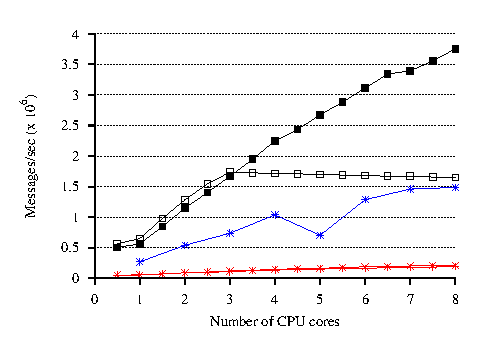
\includegraphics{figs/short-mcore-v2.eps}}
 \hspace{.01in}
 \subfloat[10GbE: $n$ roundtrips per conn. (s=64B)]{
  \label{fig:short10:roundtrips}
  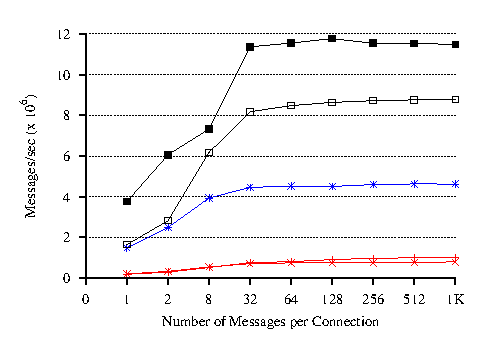
\includegraphics{figs/short-roundtrips-v2.eps}}
  \hspace{.01in}
 \subfloat[10xGbE: Different message sizes $s$ (n=1)]{
  \label{fig:short10:size}
  
\includegraphics{figs/short-size-v2.eps}}
 \centering

  \vspace{-7.8in}
  \subfloat{
\includegraphics{figs/short-key-v2.eps}}
 \vspace{7in}



\caption{Short message performance on the 10GbE and 4x10GbE setups.}
 \label{fig:shortboth}

\end{figure}


The Linux client and server implementations of our benchmarks use the
\texttt{libevent} framework with the \texttt{epoll} system call.  We
downloaded and installed mTCP from the public-domain
release~\cite{url:mtcp}, but had to write the benchmarks ourselves
using the mTCP API.  To run mTCP, we switch to the 2.6.36 kernel, as
this is the most recent supported kernel version.

\subsection{Latency and Single-flow Bandwidth}
\label{sec:eval:netpipe}

We first evaluated the latency of \ix using NetPIPE, a popular
ping-pong benchmark, using our 10GbE setup.  NetPIPE simply exchanges
a fixed-size message between two servers and helps calibrate the
latency and bandwdith of a single-flow~\cite{snell1996netpipe}.  In
all cases, the two servers use the same system (Linux, mTCP, or \ix).

%%%
%%% Numbers for latency
%% IX-IX missing
%% Linux-Linux (20.95us 
%% Linux-mTCP (86.77us)
%% mTCP-mTCP (95.53us)

Fig.~\ref{fig:pingpong} shows the goodput achieved for
different message sizes.  Two \ix servers achieve goodput of 5Gbps
(half of the maximum) with messages as small as 20KB. In
contrast, Linux requires 384KB messages to achieve 5Gbps, while
mTCP requires messages larger than 500KB. The goodput difference
between the three systems is most dramatic for small messages. Using
64B messages, the one-way latency is 6.1\microsecond between two
servers running \ix, 21\microsecond if they are running Linux, and
95\microsecond if they are running mTCP.  The differences in system
architecture explain the dramatic gap. \ix has a dataplane model
that polls queues and runs them to completion. Linux has an interrupt
model, which wakes up the blocked process. mTCP uses aggressive
batching to offset the cost of context switching~\cite{jeong2014mtcp}.

%Nevertheless, even with high message sizes, \ix maintains a \edb{2x}
%and \edb{3x} goodput advantage over mTCP and Linux respectively.
%\christos{double-check the latency numbers}

\subsection{Scalability and High Connection Churn}
\label{sec:eval:short}

%
%% put the key last to have correct numbering

\begin{figure*}

\centering
  \vspace*{0.3in}
 \subfloat[Multi-core scalability (n=1;s=64B)]{
  \label{fig:short40:mcore}
   
\includegraphics{figs/short-mcore40.eps}}
 \hspace{.01in}
 \subfloat[$n$ roundtrips per conn. (core=8,s=64B)]{
  \label{fig:short40:roundtrips}
  
\includegraphics{figs/short-roundtrips40.eps}}
  \hspace{.01in}
 \subfloat[Different message sizes $s$ (core=8,n=1)]{
  \label{fig:short40:size}
  
\includegraphics{figs/short-size40.eps}}
 \centering
  \vspace{-1.9in}
  \subfloat{
\includegraphics{figs/short-key40.eps}}
 \vspace{1.5in}
 \
\caption{Short message performance on the 4x10GbE infrastructure.}
 \label{fig:short40}

\end{figure*}


Next, we evaluate \ix's multi-core scalability in handling workloads
with extreme connection churn by using the same benchmark used to
evaluate Megapipe~\cite{han2012megapipe} and
mTCP~\cite{jeong2014mtcp}. Multiple clients connect to a single server
listening on a single port, send a request of size $s$ and wait for an
echo of a message of the same size.  As with NetPIPE, while accepting
the message, the server holds off its echo response until the message
has been entirely received.  Each client performs this synchronous
remote procedure call $n$ times, and then closes the connection using a
reset (\texttt{TCP RST}).  \dm{This begs the question of what happens
  with FIN, since that is more realistic\@.  Is the point that \ix has
an unfair advantage?}


%%
%% RAW DATA - 1024 message per connection
%% IX:  7074246
%% mTCP: 3253521

\myparagraph{10GbE results:} Figs.~\ref{fig:short10:mcore}-\ref{fig:short10:size} show the results
on the 10GbE setup.  For Linux and mTCP, our results are consistent
with the ones published in the mTCP paper~\cite{jeong2014mtcp}.  For
all three tests (core scaling, message count scaling, message size
scaling), \ix scales more aggresively and is quickly able to
saturate the hardware resources.  When reaching saturation, it is never
CPU-bound, and appears to be limited by the NIC packet per second
hardware limit (Fig.~\ref{fig:short10:mcore}) or Ethernet wire rates
limitations (Fig.~\ref{fig:short10:size}).  By contrast, \adam{new:} mTCP,
can only come close to matching \ix on Fig.~\ref{fig:short10:mcore} with all 6 cores, and
delivers 46\% of the throughput of \ix on
Fig.~\ref{fig:short10:roundtrips}.  Linux is never able to match \ix
or mTCP on any configuration.


%\subsection{High connection churn at 4x10GbE}
%\label{sec:eval:short40}


%%
%%  see data in figs/data/connection-scaling-kstats.tex
%%

\myparagraph{40GbE results:}
Figs.~\ref{fig:short40:mcore}-\ref{fig:short40:size} show the results
on the 4x10GbE setup for Linux and \ix, as well as an \ix
configuration that uses only one of the four
links. Fig.~\ref{fig:short40:mcore} shows that \ix linearly scales and
delivers 3.9MTPS on 4x10GbE with a single socket.
Fig.~\ref{fig:short40:roundtrips} shows that going to 4x10GbE also
improves throughput, but only by 30\%: the 10GbE configuration is IO
bound and within 90\% of the wire rate, resulting in small batches or
\twiddle 3 packets processed at every iteration through the \ix
pipeline.  At 4x10GbE, the workload becomes CPU bound and \ix automatically adapts to larger
pipeline batches of \twiddle 113 packets, which amortizes transitions and
improves temporal locality.  Finally, Fig.\ref{fig:short40:size} shows
that \ix can deliver 8KB messages with a goodput of 35Gbps, for a wire
throughput of 38Gpbs (out of a possible 39.7Gbps).  Overall, \ix makes
it practical to scale protected TCP/IP processing beyond 10GbE, even
with a single socket multi-core server.


\subsection{Connection Scalability}

\label{sec:eval:scale}

We also evaluate \ix's scalability when handling a large number of
concurrent connections on the 4x10GbE setup. In this benchmark, each client machine runs
$n$ threads, with each thread independently performing a 64B remote
procedure call to the server.  Each RPC randomly chooses among $m$
open sockets to perform the RPC.  In our setup with 19 clients, the
server must multiplex among $19 \times n \times m$ open connections.
We experimentally set $n \leq 24$ to maximize throughput.  We report
the maximal throughput in messages per second for varying number of
total established connections.

%Connection scaling IX/Linux @ 40Gbe 
%12036405.031689
%915256.419191
%/p
%13.15085


Fig.~\ref{fig:connscaling} shows up to to 100,000 connections, which
is the upper bound we can reach with the available client machines.
As expected, throughput increases with the degree of concurrency, but
then decreases for very large connections counts due to the
increasingly high cost of multiplexing among open connections.  At the
peak, \ix performs 13x better than Linux, consistent with the results
from Fig.~\ref{fig:short40:roundtrips}.  With 100,000 connections and
4x10GbE, \ix is able to deliver 53\% of its own peak throughput.  The
performance drop is not due to an increase in instruction counts, but
rather primarily because the size of the TCP/IP protocol control block
structures, which alone exceeds the size of the processor's layer-3
cache. \adam{new:} Moreover, there are algorithmic complexity and memory footprint overheads
in our LWIP-based TCP implementation, so we believe even greater scalability is possible.


\subsection{Memcached Performance}
\label{sec:eval:memcached}



%FIXME if different keys


\begin{figure*}[t]

\centering
  \vspace*{0.3in}
 \subfloat[Throughput for varying established connections]{
  \label{fig:connscaling:throughput}
   
\includegraphics[width=.49\textwidth,clip]{figs/blank.eps}}
 \hspace{.02in}
 \subfloat[Avg. and 99\% latency for varying established connections]{
  \label{fig:connscaling:lat}
  
\includegraphics[width=.49\textwidth,clip]{figs/blank.eps}}
\centering
  \vspace{-2.8in}
  \subfloat{
\includegraphics[width=1\textwidth,clip]{figs/short-key.eps}}
 \vspace{2.3in}
 \
\caption{Connection scaling}
 \label{fig:connscaling}

\end{figure*}

\begin{figure*}
\begin{centering}
\subfloat[Latency vs throughput for the memcached ETC workload.]{

\includegraphics{figs/memcached-etc-basic.eps}}
\subfloat[Multilate-Me Again!]{

\includegraphics{figs/blank.eps}}
\caption{Capacity and quality of service of memcached on Linux and \ix for XXX and YYY concurrent, established connections}
\label{fig:mutilate}
\end{centering}
\end{figure*}



Finally, we evaluated the performance benefits of the \ix protected
dataplane design with \texttt{memcached}, a massively deployed,
in-memory key-value store built on top of the \texttt{libevent}
framework~\cite{url:memcached}. It is frequently used as a
high-throughput, low-latency caching tier in front of persistent
database servers. \texttt{memcached} is a network-bound
application, with threads spending over 80\% of execution time in
kernel mode for network processing~\cite{Leverich:RHSU:2014}. It is a
difficult application to scale, in particular because the
common deployments involve high connection counts for
\texttt{memcached} servers and small-sized requests and
replies~\cite{nishtala2013scaling,Atikoglu:2012:WAL}

We use the \texttt{mutilate} load-generator to place a selected load
on the server in terms of requests per second (RPS) and measure
response latency~\cite{url:mutilate}. \texttt{mutilate} coordinates a
large number of client threads across multiple machines to generate
the desired RPS load, while a separate unloaded client measures
latency by issuing one request at the time.  We configure
\texttt{mutilate} to generate load representative of two workloads
from Facebook~\cite{Atikoglu:2012:WAL}: the ETC workload that
represents that highest capacity deployment in Facebook, has 20B - 70B
keys, 1B-1KB values, and 90\% GET requests; and the USR workload that
represents deployment with most GET requests in Facebook, has short
keys ($<$20B), 2B values, and 99\% GET requests. In USR, almost all
traffic involves minimum-sized TCP packets. Each request is issued 
\dm{incomplete sentence?}

\dm{Paragraph needs editing.  Also, why not report 99\% or 99.9\%?}
\adam{Are our linux graphs too noisy to do 99th? IX looks fine at 99th...}
For all experiments, we report 95th percentile latency as a function
of the achieved throughput as this is the relevant metric for
datacenter
applications\microsecond~\cite{DBLP:journals/cacm/DeanB13}. This graph
provides insights the full range of system behaviors. Most commercial
\texttt{memcached} use such a latency-throughput graph to provision
each server so that the 95th percentile latency does not exceed 200 to
500.  We carefully tune the Linux baseline setup according to the
guidelines in \cite{Leverich:RHSU:2014}. Specifically, we pin
memcached threads, configure interrupt-distribution based on
thread-affinity, and tune interrupt moderation thresholds. We believe
that our baseline Linux numbers are as tuned as possible for this
hardware using the open-source version of
\texttt{memcached-1.4.18}. For our benchmark, we use 6 client machines
and a total of 772 connections to the memcached server. We report the
results for the configuration that provides the best performance: 
8 sockets with Linux, but only 6 with \ix.

\christos{Should we discuss the porting process to IX?}
\adam{new:} Porting memcached to IX primarly consisted of adapting it
to use our event library. In most cases, the port was straightforward,
replacing Linux and \texttt{libevent} function calls with their equivalent
versions in our API. There were a few incompatibilities that required
aditional effort. For example we don't yet support vectored write
operations (e.g., \texttt{writev}) in our
API (the benefits would be only marginal because we batch
writes inside our event library). Morever, we had to make some internal changes
to memcached in order to deliniate the spawning elastic threads and background
threads.  \adam{On our haswell machine, which runs an older linux
kernel this change works great, but it had to be disabled on the mavericks and at EPFL because
newer kernels have something wierd going on with thread spawning. In pratice,
background threads didn't make any noticable difference on the Haswell. Should I say anything about this
limitation?} Finally, we made some small changes to the behavior of the main
event loop in order to better support our run to completion execution model. We
did not attempt to tune the internal scalability of memcached or adapt memcached
to support zero-copy IO operations.


%%
%% see  figs/data/memcache-sla-qps.txt

%82.5  139.6  650K
%42.0  54.3   1320K  --> 2.03x     --> 2.0x
%79.6  136.8  580K
%37.7  44.5   1620K  -->  2.74519  --> 2.7x


\begin{table}[b]
%\vspace{-1em}
\begin{center}
\begin{small}
\begin{tabular}{|l|c|c|c|}
\hline
%Configuration &  \multicolumn{2}{|c|}{Unloaded latency} &  QPS for SLA:\\
Configuration &  Minimum latency &  RPS for SLA:\\
&  @99th pct &  $<500$\microsecond@99th pct\\
\hline
ETC-Linux & 93\microsecond & 500K\\
ETC-IX    & 46\microsecond & 1500K\\
\hline
USR-Linux & 84\microsecond & 450K\\
USR-IX    & 31\microsecond & 2150K\\

\hline
\end{tabular}
\caption{Unloaded latency and maximum RPS for a given service-level agreement for the memcache workloads \texttt{ETC} and \texttt{USR}.}
%\vspace*{-2em}
\label{tbl:mutilate}
\end{small}
\end{center}
\end{table}



\edb{NEW with table:} Fig.~\ref{fig:mutilate} shows the throughput-latency curves for the
two \texttt{memcached} workloads for Linux and \ix, while
Table~\ref{tbl:mutilate} reports the unloaded latencies and maximum query throughput that meets a service-level agreement of $<1ms$ at the 95th percentile.
\ix noticeably reduces the unloaded latencies, also measured
at the 95th percentile.  We note here that the benchmark
clients are running on Linux, and that running them on \ix should
further reduce that latency. 

\edb{NEW:}For both workloads, the distribution of CPU time shifts from being
$>80\%$ in the kernel with Linux to $<30\%$ with \ix.  Since the
application is unmodified, Amdahl's law would predict a speedup of 3x.
\ix actually increases the throughput of memcached by 1.8 and 2.7
for \texttt{ETC} and \texttt{USR}, respectively.  We explain the
difference by the increased lock contention within the application
itself, in particular for \texttt{ETC}, which has a higher write frequency.


%
\subsection{Multi-tier Performance}

\edb{THIS IS A STRECH STRETCH GOAL} 

Evaluating the performance of a highly-scalable, multi-tier
environment in a lab environment is challenging on multiple fronts:
first, there are ---to the best of our knowledge--- no universally
accepted multi-tier benchmarks that involve key-value stores and in
general that are representative of web-scale applications.  Second,
most lab enviornments are orders of magnitude smaller than a
datacenter.

Therefore, we construct a simple, synthetic multi-tier benchmark that
mimics the behavior of a social application stored in an in-memory
key-value store.  The application is a simple \texttt{http} server
that returns the top-most recent update among a users list of friends.
The application server parses the http request to
get the userid, uses the user id to return a friends-list from a
key-value store, and then queries the key-value store individually for
each friend for the most recent value.  It then processes replies and
return the top-most entries.  In our experiments, we model a database
with $10^7$ million users, each with 100 friends. 

We scale the benchmark to model a cluster deployment with $\alpha$
client connections per application server, $\beta$ httpd and $\gamma$
memcached servers.  Keys are distributed uniformly between the
$\gamma$ servers.  We model a large-scale deployment with
$\alpha=10^5$, $\beta=10^4$ and $\gamma=10^4$ on a deployment that consists of 4
actual application servers and 1 memcached server (running on our
server hardware with 4x10GbE connectivity).  Each application server
runs \texttt{lighthttpd} with the application logic written directly
within the server, and maintains a distinct connection for each of the
$\alpha$ virtual clients and $\gamma$ virtual nodes.  The key-value store is
running \texttt{memcache} as described in \S\ref{sec:eval:memcache}.
We use the remaining 14 client machines to simulate $4 \times \alpha$
clients and the 19th client to measure the latency of the application.

Fig.~\ref{missing} reports the latency as a function of the
throughput, as determined by varying the client load.  We compare a
Linux baseline with one in which \ix is used to run both the
application server and the memcached server.  We note that the choice
of operating system on the application server determines the number of
concurrent connections. Indeed, because of the coherence-free
execution model, each application server needs to open a distinct TCP
flow to the same virtual node for each of its hardware threads.

\edb{OPTIMISTIC: } Fig.~\ref{missing} shows that \ix can saturate the
hardware connectivity.  Indeed, the bottlneck consits of the
communication 







